\title{Calculus-Based Physics-1: Midterm 1}
\author{Dr. Jordan Hanson - Whittier College Dept. of Physics and Astronomy}
\date{\today}
\documentclass[10pt]{article}
\usepackage[margin=1.5cm]{geometry}
\usepackage{outlines}
\usepackage{graphicx}
\usepackage{amsmath}
\usepackage{hyperref}

\begin{document}
\twocolumn

\maketitle

\section{Unit 0: Estimation, Unit \\ Analysis, Vectors, and \\ Kinematics I}

\begin{enumerate}
\item Which of the following represents a typical flow rate for a bathroom faucet?
\begin{itemize}
\item A: 0.8 liters per minute
\item A: 8.0 liters per minute
\item A: 80.0 liters per minute
\item A: 800 liters per minute
\end{itemize}
\item A train leaves Union Station in Denver, CO, heading for Chicago, IL.  If the destination is 1000 miles to the East, how long before the train arrives?
\begin{itemize}
\item A: 0.2 hours
\item B: 2.0 hours
\item C: 20.0 hours
\item D: 200.0 hours
\end{itemize}
\item What is 0.001 m s$^{-2}$ in cm min$^{-2}$?
\begin{itemize}
\item A: 3.6 km hr$^{-1}$
\item B: 36.0 km hr$^{-1}$
\item C: 360 km hr$^{-1}$
\item D: 3600 km hr$^{-1}$
\end{itemize}
\item Suppose a ship accelerates from 0 km hr$^{-1}$ to 10 km hr$^{-1}$ in 60 seconds.  What is the acceleration?
\begin{itemize}
\item A: 60 km hr$^{-1}$ s$^{-1}$
\item B: 6 km hr$^{-1}$ s$^{-1}$
\item C: 1/6 km hr$^{-1}$ s$^{-1}$
\item D: 1/60 km hr$^{-1}$ s$^{-1}$
\end{itemize}
\item Estimate the area of the North Quad of Whittier College (the open space outside the SLC):
\begin{itemize}
\item A: 5000 m$^2$
\item B: 5000 cm$^2$
\item C: 500 m$^2$
\item D: 500 cm$^2$
\end{itemize}
\item (a) Let $\vec{v} = -2\hat{i} - 2\hat{j}$, and $\vec{w} = 2\hat{i} - 2\hat{j}$.  Draw each in a 2D coordinate system below. (b) What is $\vec{v} + \vec{w}$?  (c) What is $\vec{v} - \vec{w}$? (d) What is $\vec{v} \cdot \vec{w}$? \\ \vspace{3cm}
\end{enumerate}

\section{Unit 1: Kinematics II and III}

\begin{enumerate}
\item Suppose a cyclist has a velocity of $15$ m s$^{-1}$ at $t=0$.  If the acceleration is 3 m s$^{-2}$, (a) what is the velocity at $t = 4$ seconds? (b) What is the displacement of the cyclist at $t = 4$ seconds? (c) Are the average and instantaneous velocities different at these times?  \\ \vspace{3cm}
\item Consider the motion data shown in Fig. \ref{fig:1}.  What is the acceleration of the system?
\begin{figure}
\centering
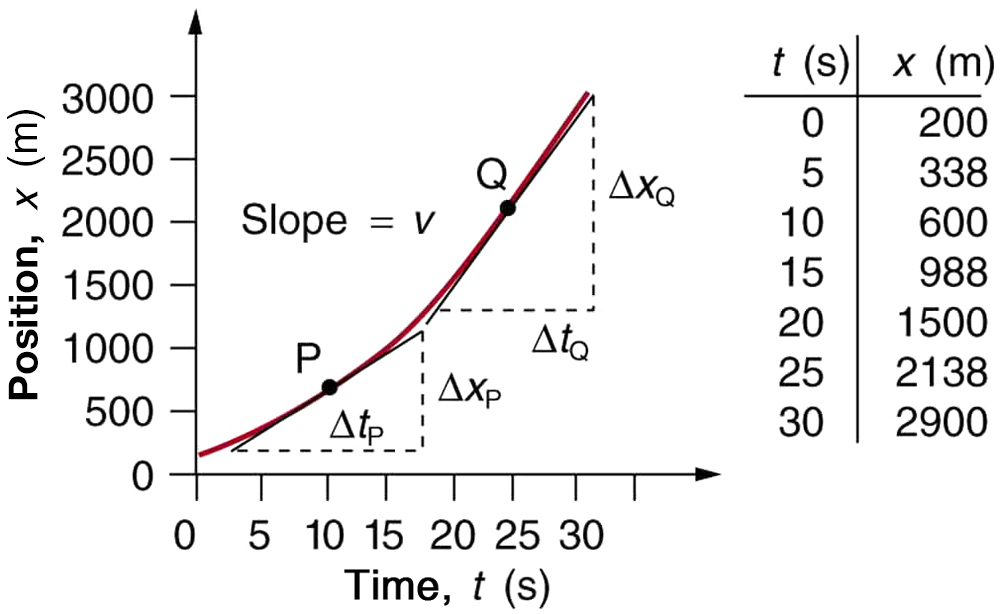
\includegraphics[width=0.4\textwidth]{slope2.jpeg}
\caption{\label{fig:1} A system moves with non-constant velocity.}
\end{figure} \vspace{3cm}
\item A system moves according to $x(t) = 12t - 3t^2$ m. (a) What is the instantaneous velocity at $t = 2$ and $t = 3$ seconds? (b) What is the average velocity between these times? (c) What is the acceleration? \\ \vspace{3cm}
\item \textbf{Design problem}.  Design an experiment in which a baseball is thrown, and the range must be 60 meters.  Choose the launch angle and initial velocity, and show that the range is 60 meters.  Provide the time of flight as well.  Finally, verify your results with the appropriate PhET simulation. \\ \vspace{3.5cm}
\item \textbf{Design problem.}  In our lab, we used a pendulum to measure $g$, the gravitational constant.  Use the following simulation to repeat that process: \url{https://phet.colorado.edu/en/simulations/pendulum-lab}. Recall that the formula relating period $T$ to $g$ is $T = 2\pi\sqrt{L/g}$, where $L$ is the pendulum length. Show your work in the form of a (handwritten) graph and relevant calculuations. \\ \vspace{3.5cm}
\end{enumerate}

\section{Unit 2: Forces I and II}

\begin{enumerate}
\item Consider the uniform circular motion depicted in Fig. \ref{fig:2}. (a) Derive expressions for the position, velocity, and acceleration of the sytem. (b) A proton is trapped in a particle accelerator and goes around the circle in $T = 200$ ns.  What is the frequency of the rotation, $f = 1/T$? (c) Convert this to \textit{angular frequency}, $\omega = 2\pi f$. (d) If the radius of the circle is $r=1$ m, and the position of the proton is $\vec{r}(0) = 1\hat{i}$ m at $t=0$, where is the proton at $t=700$ ns? (d) Look up the mass of the proton in kg, and compute the centripetal force required for this system.
\begin{figure}
\centering
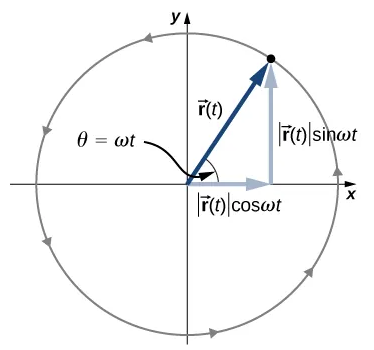
\includegraphics[width=0.35\textwidth]{circ_motion.png}
\caption{\label{fig:2} Uniform circular motion.}
\end{figure} \vspace{3.5cm}
\item A 14,500 kg F/A-18 Super Hornet lands on an aircraft carrier, moving at 230 km hr$^{-1}$. A tow cable grabs the aircraft and pulls it to a stop in 330 meters. (a) What is the average acceleration? (b) What force does the tow cable extert to stop the jet? \\ \vspace{2.5cm}
\item Two children pull a third child on a snow saucer sled exerting forces $\vec{F}_1$ and $\vec{F}_2$ as shown in Fig. \ref{fig:3}. Find the acceleration of the 36 kg sled and child system.
\begin{figure}
\centering
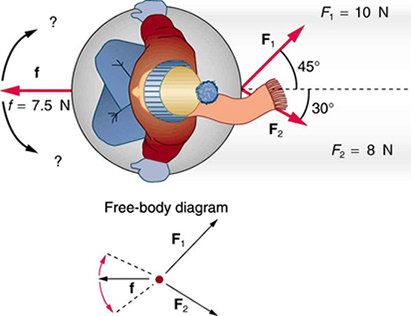
\includegraphics[width=0.425\textwidth]{sled.jpeg}
\caption{\label{fig:3} Two people pull on a third person on a sled, on an icy surface.}
\end{figure}\vspace{2cm}
\end{enumerate}

\begin{enumerate}
\item Now consider the sled and child in the previous exercise, sliding down a hill with the friction coefficient for steel on ice ($\mu=0.02$).  (a) If the hill has a 10 degree incline, what is the acceleration? (b) How far will the child and sled travel in 20 seconds? \\ \vspace{3cm}
\item Consider four springs connected \textit{in parallel} to an object of mass $m$.  Each spring has a spring constant $k$, and each spring is attached to the floor and the object. (a) Draw a free-body diagram. (b) Derive an expression for the displacement of the springs. (c) Show that, in the limit that $k \to \infty$, the displacement goes to zero.  This is a basic model for vehicle suspension. (d) Verify your results with the Hooke's Law PhET simulation.  Show that two springs \textit{in parallel} with the same k-value act as one spring with twice the k-value.  \\ \vspace{4cm}
\item What is the terminal velocity of a 60 kg skydiver with area $A = 0.25$ m$^2$, and drag coefficient $C = 0.5$?  Use the standard density of air: $\rho = 1.2$ kg m$^{-3}$. (b) What is the terminal velocity if she opens the parachute, increasing the cross-sectional area by a factor of 100? \\ \vspace{3cm}
\end{enumerate}

\section{Unit 3: Work and Energy}

\begin{enumerate}
\item A force $\vec{F} = -2\hat{i} - 1\hat{j}$ N acts on a system in the xy-plane.  (a) Calculate the work done on the system, if $\vec{x}_i = 2\hat{i} + 2\hat{j}$ and $\vec{x}_f = -2\hat{i} - 2\hat{j}$. (b) What is the final kinetic energy if the system started from rest?  (c) If the mass is 0.5 kg, what is the final velocity? \\ \vspace{4cm}
\item \textbf{Design problem.} (a) Design a spring launcher system that accelerates a 3 gram marble to 8 m s$^{-1}$.  What k-value do you choose, and what displacement is required for the spring? (b) If your spring launcher is oriented at a 45 degree angle above the horizontal, where will the marble land? (c) Verify your results with the Projectile Motion PhET simulation.  Set the speed and angle correctly, and measure the range. (d) Draw a graph of the trajectory of the marble.
\end{enumerate}

\end{document}